\section{Results}
\label{sec:results}
\subsection{Discrimination across four training seeds}
All 60 runs of the three principal models completed training and formal evaluation. Sixty evaluation receipts and 180 registered report identities were verified. Every seed-specific predictor averaged five fold probabilities for each of the same 175 holdout patients, including 56 positive outcomes. We then calculated metrics within each seed and averaged the metrics across seeds 42, 44, 71, and 2026. Table~\ref{tab:main} reports means with sample seed standard deviations; conditional patient intervals and paired tests are reported separately.
\begin{table*}[t]
\centering
\small
\caption{Performance on the fixed internal holdout (175 patients, 56 pCR positive). Entries are mean $\pm$ sample SD over seeds 42, 44, 71, and 2026. Within each seed, five fold probabilities are averaged per patient before metrics; no probabilities are averaged across seeds. Macro averages T0--T2 metrics within each seed. F1 uses threshold 0.5. Paired Macro differences and adjusted tests are in Table~\ref{tab:bootstrap}.}
\label{tab:main}
\begin{tabular}{llrrr}
\toprule
Model & Landmark & AUROC & AP & F1 \\
\midrule
NoJEPA & T0 & 0.7270 $\pm$ 0.0037 & 0.5898 $\pm$ 0.0092 & 0.5332 $\pm$ 0.0152 \\
NoJEPA & T1 & 0.7251 $\pm$ 0.0054 & 0.5911 $\pm$ 0.0093 & 0.5399 $\pm$ 0.0107 \\
NoJEPA & T2 & 0.7254 $\pm$ 0.0051 & 0.5907 $\pm$ 0.0076 & 0.5416 $\pm$ 0.0166 \\
NoJEPA & Macro & 0.7258 $\pm$ 0.0044 & 0.5905 $\pm$ 0.0086 & 0.5382 $\pm$ 0.0138 \\
DirectReadout & T0 & 0.7341 $\pm$ 0.0089 & 0.5932 $\pm$ 0.0091 & 0.5392 $\pm$ 0.0189 \\
DirectReadout & T1 & 0.7369 $\pm$ 0.0107 & 0.6010 $\pm$ 0.0145 & 0.5388 $\pm$ 0.0261 \\
DirectReadout & T2 & 0.7353 $\pm$ 0.0071 & 0.5975 $\pm$ 0.0123 & 0.5556 $\pm$ 0.0097 \\
DirectReadout & Macro & 0.7354 $\pm$ 0.0087 & 0.5972 $\pm$ 0.0107 & 0.5446 $\pm$ 0.0176 \\
ForecastMean & T0 & 0.7476 $\pm$ 0.0060 & 0.6162 $\pm$ 0.0159 & 0.5739 $\pm$ 0.0130 \\
ForecastMean & T1 & 0.7494 $\pm$ 0.0070 & 0.6205 $\pm$ 0.0138 & 0.5821 $\pm$ 0.0149 \\
ForecastMean & T2 & 0.7478 $\pm$ 0.0076 & 0.6225 $\pm$ 0.0123 & 0.5719 $\pm$ 0.0036 \\
ForecastMean & Macro & 0.7483 $\pm$ 0.0067 & 0.6197 $\pm$ 0.0137 & 0.5760 $\pm$ 0.0083 \\
\bottomrule
\end{tabular}
\end{table*}


\fullmodel{} had mean T0/T1/T2 AUROCs of 0.7476/0.7494/0.7478 and AP values of 0.6162/0.6205/0.6225 (Fig.~\ref{fig:discrimination}). Its Macro AUROC/AP/F1 was 0.7483/0.6197/0.5760, with sample seed standard deviations of 0.0067/0.0137/0.0083. Corresponding means were 0.7258/0.5905/0.5382 for \nojepa{} and 0.7354/0.5972/0.5446 for \direct{}. Forecast mean had the highest mean AUROC, AP, and F1 at every landmark among the three reported models. Its T2 F1 was 0.5719, compared with 0.5556 for \direct{} and 0.5416 for \nojepa{}. These are averages of metrics from four separately evaluated seed-specific ensembles, not metrics of a combined predictor.

\begin{figure*}[t]
\centering
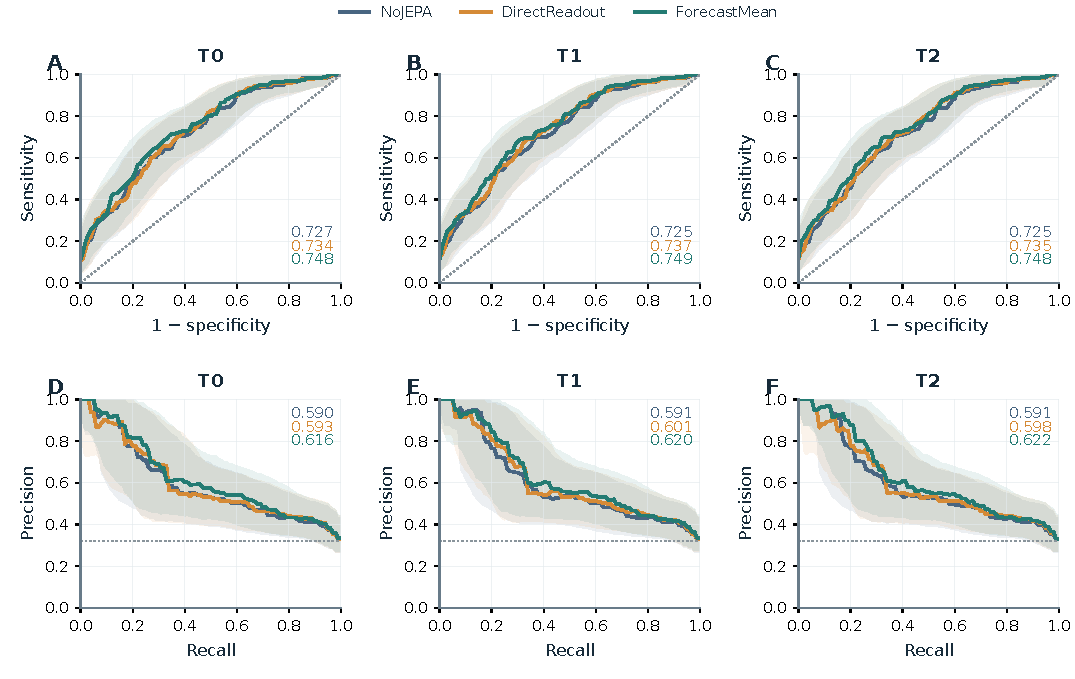
\includegraphics[width=\textwidth]{figures/discrimination.pdf}
\caption{Discrimination across seeds 42, 44, 71, and 2026. (A--C) Mean ROC curves; (D--F) mean precision--recall curves. Curves are computed from five-fold ensemble probabilities separately within each seed, interpolated on a common grid, and equally averaged across seeds. Shading gives pointwise conditional 95\% shared-patient-bootstrap intervals for the mean curve. Colored metric values are means of the directly computed seed-specific AUROC or non-interpolated AP; they need not equal the area under the displayed mean curve. The dotted PR reference is the 0.32 positive prevalence.}
\label{fig:discrimination}
\end{figure*}

Under direct readout, adding future-state supervision increased mean Macro AUROC/AP/F1 by +0.0096/+0.0067/+0.0063. Adding the complete mean forecast readout increased these means by a further +0.0129/+0.0225/+0.0314 relative to \direct{}. These means conceal variation among seeds. The direct-versus-\nojepa{} Macro AUROC comparison was negative at seed 2026 (0.7230 versus 0.7251). Forecast mean had lower AUROC than \direct{} at seed 42 (0.7407 versus 0.7428), despite higher AP and F1. Its Macro AUROC/AP/F1 at seed 71 was 0.7569/0.6394/0.5869; the corresponding direct-readout values were 0.7358/0.5825/0.5369. The full-versus-\nojepa{} Macro AUROC difference was positive at all four selected seeds. The supplementary seed tables retain each realization, including the unfavorable contrasts; the selected subset does not establish behavior across all possible seeds.


Paired patient intervals qualify the descriptive rankings (Fig.~\ref{fig:paired}). The mean Macro AUROC difference for \fullmodel{} versus \nojepa{} was +0.0225 [0.0106, 0.0347]. The corresponding \direct{}--\nojepa{} difference was +0.0096 [0.0002, 0.0193], and the \fullmodel{}--\direct{} difference was +0.0129 [0.0021, 0.0236]. The full-versus-\nojepa{} AP/F1 differences were +0.0292 [0.0078, 0.0508] and +0.0377 [0.0034, 0.0782]. Against \direct{}, they were +0.0225 [0.0043, 0.0411] and +0.0314 [0.0003, 0.0697]. These unadjusted intervals concern patient sampling conditional on the selected fitted predictors and are distinct from descriptive seed standard deviations or multiplicity-adjusted tests.

The full-versus-\nojepa{} Macro AUROC difference had approximate paired-bootstrap raw $p=0.00050$, nine-test Holm $p=0.00450$, and all-78 Holm $p=0.03850$. It was the only principal comparison meeting the family-adjusted 0.05 criterion. The corresponding AP and F1 comparisons had raw/within-family adjusted $p=0.01020/0.08160$ and 0.04513/0.22565, respectively. All three full-versus-direct Macro comparisons remained nonsignificant after principal-family adjustment: AUROC/AP/F1 adjusted values were 0.13699/0.13699/0.22565. The auxiliary-supervision AUROC comparison also did not pass adjustment (raw $p=0.04678$, adjusted 0.22565). Nonsignificance does not establish equivalence.

Within the secondary family, only the full-versus-\nojepa{} T1 and T2 AUROC differences met the adjusted criterion. T1 had a difference of +0.0243 [0.0117, 0.0372], raw $p=0.00036$, secondary-family Holm $p=0.02484$, and all-78 Holm $p=0.02808$. T2 had a difference of +0.0224 [0.0100, 0.0353], raw $p=0.00058$, secondary-family Holm $p=0.03944$, and all-78 Holm $p=0.04408$. The Macro, T1, and T2 AUROC contrasts were the only three comparisons meeting the all-78 criterion. They remain conditional on the retrospectively selected predictors and reporting policy.

The independent 999,999-resample T2 AUROC check yielded raw $p=0.000722$ with Monte Carlo standard error approximately 0.0000269. Replacing only this entry and holding the other 77 values fixed gave secondary-family Holm $p=0.049096$ and all-78 Holm $p=0.054872$. Thus the T2 all-78 decision crossed the 0.05 threshold relative to the uniform-table value 0.04408; it should not be interpreted as robust to numerical precision. Macro and T1 retain their original values in this sensitivity calculation, but their bootstrap simulations were not repeated. The main table continues to report the uniform 99,999-resample analysis.
\begin{table*}[t]
\centering
\small
\caption{Exploratory principal Macro comparisons. All metrics use approximate, null-centered paired patient-bootstrap tests with 99,999 shared resamples. Within each draw, metrics are computed for each seed then equally averaged. All $p$ values are two-sided. Holm$_9$ adjusts the nine entries here; Holm$_{78}$ is the sensitivity analysis over all 78 principal and secondary tests. Sig. refers to Holm$_9$. Direct and Mean abbreviate DirectReadout and ForecastMean. $^{*}p_{\mathrm{Holm}}<0.05$, $^{**}p_{\mathrm{Holm}}<0.01$, $^{***}p_{\mathrm{Holm}}<0.001$; ns, not significant after the stated correction. Intervals are unadjusted 95\% patient-bootstrap intervals (2,000 shared draws) and need not agree with adjusted test decisions. All analyses condition on the fixed, retrospectively selected seed42/44/71/2026 ensembles; seeds are not resampled.}
\label{tab:bootstrap}
\begin{tabular}{llrrrrc}
\toprule
Comparison & Metric & Difference [95\% CI] & $p$ & $p_{\mathrm{Holm},9}$ & $p_{\mathrm{Holm},78}$ & Sig. \\
\midrule
Direct -- NoJEPA & AUROC & +0.0096 [+0.0002, +0.0193] & 0.0468 & 0.2257 & 1.0000 & ns \\
Direct -- NoJEPA & AP & +0.0067 [-0.0055, +0.0203] & 0.3092 & 0.6185 & 1.0000 & ns \\
Direct -- NoJEPA & F1 & +0.0063 [-0.0098, +0.0216] & 0.4079 & 0.6185 & 1.0000 & ns \\
Mean -- NoJEPA & AUROC & +0.0225 [+0.0106, +0.0347] & 0.0005 & 0.0045 & 0.0385 & ** \\
Mean -- NoJEPA & AP & +0.0292 [+0.0078, +0.0508] & 0.0102 & 0.0816 & 0.7140 & ns \\
Mean -- NoJEPA & F1 & +0.0377 [+0.0034, +0.0782] & 0.0451 & 0.2257 & 1.0000 & ns \\
Mean -- Direct & AUROC & +0.0129 [+0.0021, +0.0236] & 0.0202 & 0.1370 & 1.0000 & ns \\
Mean -- Direct & AP & +0.0225 [+0.0043, +0.0411] & 0.0196 & 0.1370 & 1.0000 & ns \\
Mean -- Direct & F1 & +0.0314 [+0.0003, +0.0697] & 0.0730 & 0.2257 & 1.0000 & ns \\
\bottomrule
\end{tabular}
\end{table*}


\begin{figure*}[t]
\centering
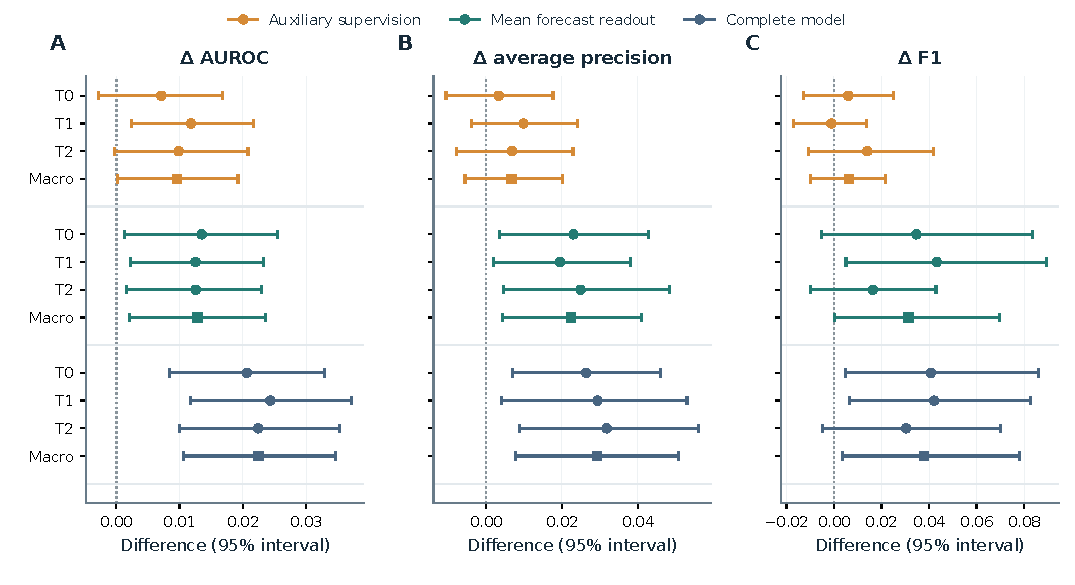
\includegraphics[width=\textwidth]{figures/paired_comparisons.pdf}
\caption{Paired seed-mean metric differences at T0, T1, T2, and Macro. Colors distinguish auxiliary supervision, additional forecast readout, and the complete-model contrast. Squares denote Macro estimates. Bars are unadjusted 95\% patient-bootstrap intervals. Every draw is shared across seeds, models, and landmarks; metrics are computed within seed before averaging. Adjusted tests appear in Tables~\ref{tab:bootstrap} and~\ref{tab:significance_landmarks}. Folds, seeds, and repeated landmarks do not create independent test cohorts.}
\label{fig:paired}
\end{figure*}

\subsection{Threshold behavior and class imbalance}
\begin{table*}[t]
\centering
\small
\caption{Operating characteristics at threshold 0.5. Entries average the four seed-specific fivefold probability-ensemble metrics; Macro first averages T0--T2 within each seed. The same 175 patients appear in every evaluation.}
\label{tab:extended_operating}
\begin{tabular}{llrrrrrr}
\toprule
Model & Landmark & Sens. & Spec. & PPV & NPV & BA & MCC \\
\midrule
NoJEPA & T0 & 0.580 & 0.721 & 0.496 & 0.786 & 0.650 & 0.291 \\
NoJEPA & T1 & 0.598 & 0.710 & 0.494 & 0.790 & 0.654 & 0.296 \\
NoJEPA & T2 & 0.603 & 0.708 & 0.493 & 0.792 & 0.655 & 0.297 \\
NoJEPA & Macro & 0.594 & 0.713 & 0.494 & 0.789 & 0.653 & 0.295 \\
\midrule
DirectReadout & T0 & 0.576 & 0.737 & 0.510 & 0.787 & 0.657 & 0.305 \\
DirectReadout & T1 & 0.580 & 0.731 & 0.505 & 0.788 & 0.656 & 0.302 \\
DirectReadout & T2 & 0.634 & 0.695 & 0.495 & 0.802 & 0.665 & 0.313 \\
DirectReadout & Macro & 0.597 & 0.721 & 0.503 & 0.792 & 0.659 & 0.307 \\
\midrule
ForecastMean & T0 & 0.674 & 0.683 & 0.500 & 0.817 & 0.678 & 0.336 \\
ForecastMean & T1 & 0.679 & 0.693 & 0.510 & 0.821 & 0.686 & 0.351 \\
ForecastMean & T2 & 0.683 & 0.668 & 0.492 & 0.818 & 0.676 & 0.330 \\
ForecastMean & Macro & 0.679 & 0.681 & 0.501 & 0.819 & 0.680 & 0.339 \\
\bottomrule
\end{tabular}
\end{table*}

At threshold 0.5, mean Macro sensitivity/NPV was 0.6786/0.8186 for \fullmodel{}, compared with 0.5967/0.7924 for \direct{}. These increases accompanied lower specificity (0.6814 versus 0.7213) and slightly lower PPV (0.5008 versus 0.5033). The paired mean sensitivity difference was +0.0818 [0.0404, 0.1327], while the specificity difference was $-0.0399$ [$-0.0663$, $-0.0165$]. Relative to \nojepa{}, sensitivity increased by +0.0848 [0.0396, 0.1398] and specificity decreased by $-0.0315$ [$-0.0603$, $-0.0057$]. These unadjusted intervals describe an operating trade-off. Against \direct{}, raw/secondary-family adjusted $p$ values were 0.00127/0.08509 for sensitivity and 0.00191/0.12415 for specificity. No operating or probability-quality comparison met the secondary-family adjusted criterion.



The full model's seed-mean true-positive counts at T0/T1/T2 were 37.75/38.00/38.25, with false-positive counts 37.75/36.50/39.50. These are averages of integer counts from four correlated predictors, not fractional patients or a single combined confusion matrix. Mean F1 increased from 0.5739 at T0 to 0.5821 at T1, then decreased to 0.5719 at T2. The additional T2 positive predictions included more false positives, illustrating why further observations need not improve a fixed-threshold decision rule.

\fullmodel{} had the highest mean Macro balanced accuracy (0.6800) and MCC (0.3391), compared with 0.6590/0.3066 for \direct{} and 0.6533/0.2947 for \nojepa{}. Accuracy was 0.6814 for \direct{}, 0.6805 for forecast mean, and 0.6748 for \nojepa{}. The first two means were only slightly above the all-negative reference of 0.68. Accuracy, ranking, and class-specific errors therefore give different descriptive orderings.

OOF-selected Youden thresholds changed mean holdout Macro F1 from 0.5382 to 0.5418 for \nojepa{}, 0.5446 to 0.5420 for \direct{}, and 0.5760 to 0.5743 for \fullmodel{} (Table~\ref{tab:extended_threshold}). Thus the alternative threshold produced a small increase for \nojepa{} and decreases for the other models. These results concern transfer of thresholds fitted on single-model OOF scores to within-seed five-model ensemble scores; they neither optimize a holdout threshold nor establish independent ensemble calibration.

\subsection{Longitudinal information and probability quality}
The paired seed-mean T2--T0 AUROC change was +0.0002 [$-0.0054$, 0.0061] for \fullmodel{}, $-0.0016$ [$-0.0064$, 0.0029] for \nojepa{}, and +0.0011 [$-0.0034$, 0.0057] for \direct{}. The full model's corresponding AP change was +0.0062 [$-0.0063$, 0.0194] and F1 change $-0.0020$ [$-0.0125$, 0.0095]. All these longitudinal intervals included zero. Forecast mean's AUROC was highest at T1, whereas mean AP increased across landmarks; neither pattern establishes a confirmed benefit from an additional visit. Fig.~\ref{fig:scorechanges} shows outcome-conditioned distributions of changes in seed-specific ensemble probabilities.

\begin{table*}[t]
\centering
\small
\caption{Probability quality: four-seed mean $\pm$ sample SD of Macro metrics. Each seed has its own fivefold probability ensemble. Lower is better; ECE uses ten equal-width bins.}
\label{tab:calibration}
\begin{tabular}{lrrr}
\toprule
Model & NLL & Brier & ECE \\
\midrule
NoJEPA & 0.5812 $\pm$ 0.0081 & 0.1996 $\pm$ 0.0036 & 0.1157 $\pm$ 0.0196 \\
DirectReadout & 0.5771 $\pm$ 0.0104 & 0.1979 $\pm$ 0.0045 & 0.1207 $\pm$ 0.0204 \\
ForecastMean & 0.5829 $\pm$ 0.0118 & 0.2002 $\pm$ 0.0054 & 0.1405 $\pm$ 0.0178 \\
\bottomrule
\end{tabular}
\end{table*}

Mean Macro NLL/Brier/ECE was 0.5829/0.2002/0.1405 for \fullmodel{}, compared with 0.5771/0.1979/0.1207 for \direct{} and 0.5812/0.1996/0.1157 for \nojepa{}. Forecast mean had worse point estimates of all three probability-quality metrics than both direct-readout controls. The higher discrimination means therefore did not translate into better probability-quality means. All 14 Macro metrics and their conditional patient intervals appear in Table~\ref{tab:extended_macro}.

\begin{figure*}[t]
\centering
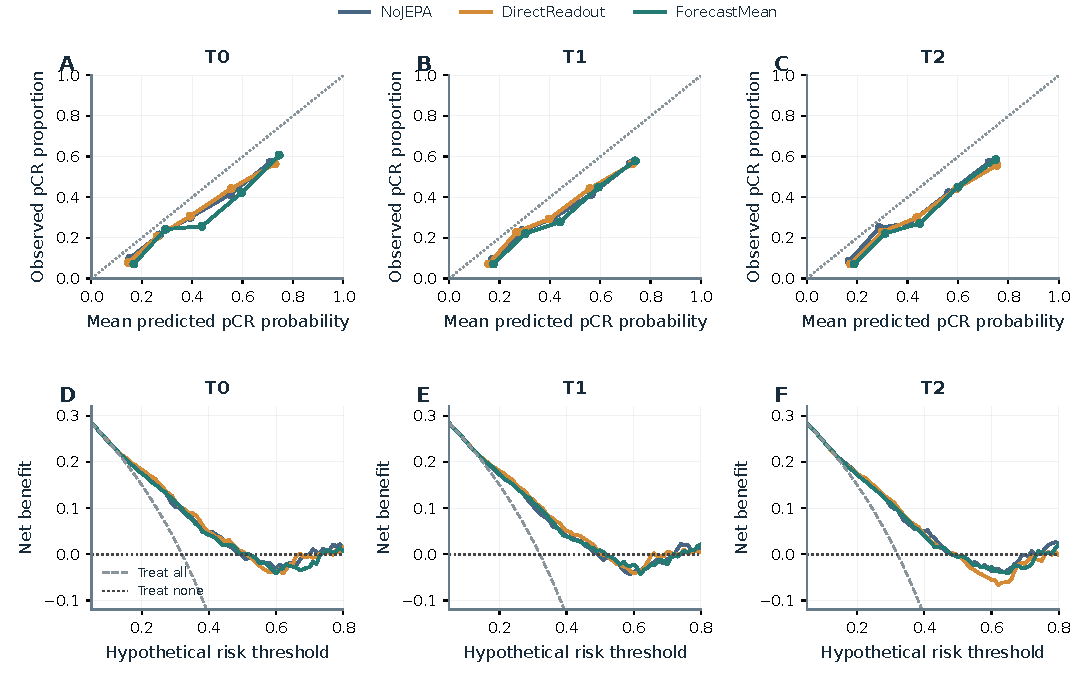
\includegraphics[width=\textwidth]{figures/calibration_utility.pdf}
\caption{Probability quality and hypothetical decision utility across four seeds. (A--C) Reliability summaries first form five equal-count probability-rank groups of 35 patients within each seed-specific five-fold ensemble and then average the group summaries across seeds. They differ from the ten equal-width bins used for ECE. (D--F) Net-benefit curves are computed separately within seeds and then averaged, with treat-all and treat-none references. Scores are not recalibrated. No clinical escalation or de-escalation strategy is validated.}
\label{fig:calutility}
\end{figure*}

\subsection{Hypothetical net benefit}
Decision curves did not preserve the discrimination ranking across thresholds. At a hypothetical threshold of 0.30, mean Macro net benefit was 0.1169 for \direct{} and 0.1118 for \fullmodel{}. At 0.50, it was $-0.0052$ for \nojepa{}, +0.0014 for \direct{}, and +0.0005 for \fullmodel{}. At 0.70, forecast mean had lower net benefit ($-0.0267$) than direct readout ($-0.0067$). These values average seed-specific decision curves, use uncalibrated probabilities, and assume a generic positive action. They do not establish an acceptable clinical threshold or validate a management pathway.

\subsection{Exploratory biological and acquisition-related subgroups}
The four HR/HER2 groups had positive seed-mean Macro AUROC differences between \fullmodel{} and \nojepa{} (Fig.~\ref{fig:subgroups}; Table~\ref{tab:subgroups}). The HR-positive/HER2-negative group had a difference of +0.0385 [0.0089, 0.0743] among 68 patients, including 11 positive outcomes. Other differences were +0.0143 [$-0.0349$, 0.0629] in HR-positive/HER2-positive patients (31, 12 positive), +0.0272 [$-0.0272$, 0.1136] in HR-negative/HER2-positive patients (14, 7 positive), and +0.0380 [0.0083, 0.0705] in HR-negative/HER2-negative patients (62, 26 positive). The first and fourth groups' unadjusted intervals excluded zero. These exploratory intervals do not establish a multiplicity-adjusted subtype benefit or an interaction.

In the HR-positive/HER2-negative group, forecast mean's mean Macro sensitivity/specificity was 0.1515/0.9620, compared with 0.1061/0.9868 for \nojepa{}. Thus low sensitivity at threshold 0.5 persisted despite the positive AUROC difference. \direct{} had sensitivity/specificity 0.0985/0.9912. Mean Macro AUROC was 0.7197 for forecast mean, 0.7064 for \direct{}, and 0.6812 for \nojepa{}. Age-group summaries remain exploratory and do not support an age-interaction conclusion. Source namespaces share one clinical release and do not constitute external validation. The partially clipped baseline-component group contained only 11 patients and one positive outcome; its AUROC and AP were suppressed under the minimum-outcome rule.

\begin{figure*}[t]
\centering
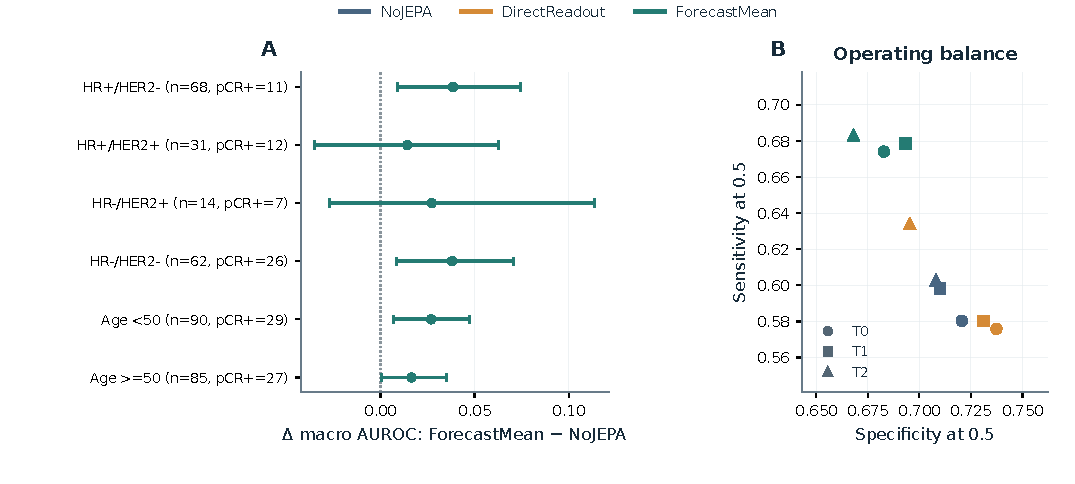
\includegraphics[width=\textwidth]{figures/subgroup_operating.pdf}
\caption{Exploratory subgroup and operating-point summaries, with metrics computed within seed and then equally averaged across seeds 42, 44, 71, and 2026. (A) Macro AUROC differences between ForecastMean and NoJEPA within HR/HER2 and age groups, with patient counts, positive outcomes, and unadjusted shared-patient intervals. No subgroup-interaction claim is made. (B) Mean specificity and sensitivity at threshold 0.5 across landmarks; colors identify models and markers identify landmarks.}
\label{fig:subgroups}
\end{figure*}

\subsection{Archived forecast and gradient diagnostics}
Archived fixed-training-probe diagnostics describe individual models separately from the pCR holdout analysis (Fig.~\ref{fig:mechanism}). At common epoch 20, mean copy-normalized forecast skills for \direct{} were +0.0129, +0.0621, and +0.1635 at one-, two-, and three-step horizons. Corresponding values for \fullmodel{} were $-0.0469$, $-0.0479$, and +0.0283 (Table~\ref{tab:worldprobe}). Statistics were normalized within each snapshot's EMA coordinates, averaged across five folds within seed, and then averaged across four seeds. Separate models' latent states were not ensembled. These diagnostics do not support attributing forecast mean's pCR ranking to uniformly more accurate latent forecasts.

The probe requires the real landmark, target, and every intermediate examination, whereas the training objective masks unavailable future targets. Eligible populations therefore vary by horizon; only 5--9 patients per probe were eligible at three steps. These measurements are not selected-checkpoint holdout forecast evaluations. The predictor's pCR-loss gradient norm was zero for \direct{} and had mean 0.9867 for \fullmodel{}; weighted rollout-gradient means were 0.1474 and 0.1715. These values support the expected gradient routing, but gradient magnitude is not a biological effect size. \nojepa{} had no available trained-world diagnostic and was not assigned an artificial zero skill.

\begin{figure*}[t]
\centering
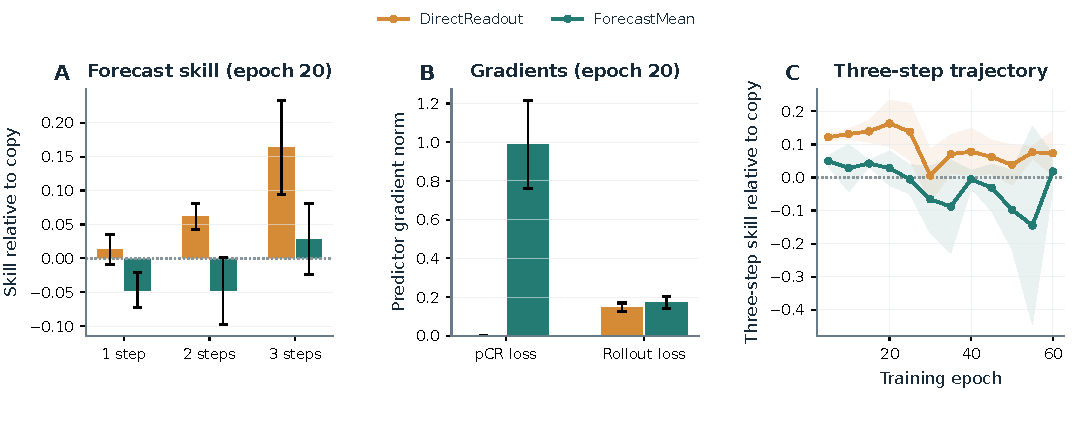
\includegraphics[width=\textwidth]{figures/forecast_mechanism.pdf}
\caption{Archived fixed-training-probe diagnostics across four seeds. (A) Copy-normalized forecast skill at common epoch 20. (B) Predictor gradient norms from pCR and weighted rollout losses. (C) Three-step skill across epochs with complete diagnostic coverage. Statistics are calculated within each snapshot's EMA coordinates, averaged across folds within seed, and summarized across seeds. Error bars in A and B and shading in C show the descriptive sample SD of the four seed-specific fold means. These are training diagnostics, distinct from pCR probability ensembling; real continuous visit chains are required, and three-step eligibility is only 5--9 patients per probe.}
\label{fig:mechanism}
\end{figure*}
